%% This is file `elsarticle-template-1-num.tex',
%%
%% Copyright 2009 Elsevier Ltd
%%
%% This file is part of the 'Elsarticle Bundle'.
%% ---------------------------------------------
%%
%% It may be distributed under the conditions of the LaTeX Project Public
%% License, either version 1.2 of this license or (at your option) any
%% later version.  The latest version of this license is in
%%    http://www.latex-project.org/lppl.txtt
%% and version 1.2 or later is part of all distributions of LaTeX
%% version 1999/12/01 or later.
%%
%% The list of all files belonging to the 'Elsarticle Bundle' is
%% given in the file `manifest.txt'.
%%
%% Template article for Elsevier's document class `elsarticle'
%% with numbered style bibliographic references
%%
%% $Id: elsarticle-template-1-num.tex 149 2009-10-08 05:01:15Z rishi $
%% $URL: http://lenova.river-valley.com/svn/elsbst/trunk/elsarticle-template-1-num.tex $
%% Step
%\documentclass[preprint,12pt]{elsarticle}
%\documentclass[nofootinbib,12pt]{revtex4}
%% Use the option review to obtain double line spacing
% \documentclass[preprint,review,12pt]{elsarticle}

%% Use the options 1p,twocolumn; 3p; 3p,twocolumn; 5p; or 5p,twocolumn
%% for a journal layout:
%\documentclass[final,1p,times]{elsarticle}
%\documentclass[final,1p,times,twocolumn]{elsarticle}
%%\documentclass[final,3p,times]{elsarticle}
% This is the NIM format
\documentclass[final,3p,times,twocolumn]{elsarticle}

%% if you use PostScript figures in your article
%% use the graphics package for simple commands
%% \usepackage{graphics}
%% or use the graphicx package for more complicated commands
%% \usepackage{graphicx}
%% or use the epsfig package if you prefer to use the old commands
%% \usepackage{epsfig}

%% The amssymb package provides various useful mathematical symbols
\usepackage{amssymb}
%% The amsthm package provides extended theorem environments
\usepackage{amsthm}
\usepackage[figuresright]{rotating}
\usepackage{hyperref}
\usepackage{subfig}
%% The lineno packages adds line numbers. Start line numbering with
%% \begin{linenumbers}, end it with \end{linenumbers}. Or switch it on
%% for the whole article with \linenumbers after \end{frontmatter}.

\usepackage{lineno}
\usepackage{natbib}
%% natbib.sty is loaded by default. However, natbib options can be
%% provided with \biboptions{...} command. Following options are
%% valid:

%%   round  -  round parentheses are used (default)
%%   square -  square brackets are used   [option]
%%   curly  -  curly braces are used      {option}
%%   angle  -  angle brackets are used    <option>
%%   semicolon  -  multiple citations separated by semi-colon
%%   colon  - same as semicolon, an earlier confusion
%%   comma  -  separated by comma
%%   numbers-  selects numerical citations
%%   super  -  numerical citations as superscripts
%%   sort   -  sorts multiple citations according to order in ref. list
%%   sort&compress   -  like sort, but also compresses numerical citations
%%   compress - compresses without sorting
%%
%% \biboptions{comma,round}
\usepackage{lipsum}
% \biboptions{}

% HPS stuff
\usepackage{color}
%\usepackage{multicol}
\newcommand{\Aprime}{A\ensuremath{^\prime}}
\newcommand{\ee}{e$^+$e$^-$}
\newcommand{\fluenceunit}{1~MeV~neutron~equivalent/cm\ensuremath{^2}}
\newcommand{\geant}{{\sc Geant4}}
\newcommand{\egs}{{\sc EGS5}}
\newcommand{\moliere}{Moli\`{e}re}
%\include{affiliations}

%\journal{Nuclear Physics B}

\begin{document}

\begin{frontmatter}

%% Title, authors and addresses

\title{The CLAS12 Beamline and its Performance}

%%%%%%%%%%%%%%%%%%%%%%%%%%%%%%%%%%%%%%%%%%%%%%%%%%
%% use optional labels to link authors explicitly to addresses:
%% \author[label1,label2]{<author name>}
%% \address[label1]{<address>}
%% \address[label2]{<address>}

\newcommand{\red[1]}{{\color{red}{\bf #1}}}
\newcommand{\JLAB}{Thomas Jefferson National Accelerator Facility, Newport News, Virginia 23606}
\newcommand{\ODU}{Old Dominion University, Norfolk, Virginia 23529}
\newcommand{\UNH}{University of New Hampshire, Department of Physics, Durham, NH 03824}
\newcommand{\FIU}{Florida International University, Miami, FL 33199}
\newcommand{\INFN}{INFN, Sezione di Genova, Via Dodecaneso 33, I-16146, Genova, Italy}
\newcommand{\YERPHI}{A. Alikhanian National Laboratory, Yerevan, Armenia}
\newcommand{\KOR}{Kyungpook National University, 80 Daehakro, Daegu 41566 Korea}
\newcommand{\UCONN}{University of Connecticut, Storrs, CT 06269-3046}

\author[JLAB]{N. Baltzell}
\author[JLAB]{V.D. Burkert}
\author[FIU]{J. Carvajal}
\author[YERPHI]{N. Dashyan}
\author[INFN]{R. De Vita}
\author[JLAB]{L. Elouadrhiri} 
\author[JLAB]{G. Kharashvili}
\author[UCONN]{~~~A. Kim}
\author[UNH]{R. Paremuzyan}
\author[FIU]{B.A. Raue}
\author[JLAB]{S. Stepanyan}
%\author[KOR]{ J. A. Tan}
\author[JLAB]{M. Ungaro}
\author[FIU]{K. Wild} 
%\author[ODU]{H. Vance}
%

\address[JLAB]{\JLAB}
\address[YERPHI]{\YERPHI}
\address[INFN]{\INFN}
\address[UCONN]{\UCONN}
\address[UNH]{\UNH}
\address[FIU]{\FIU}     
%\address[KOR]{\KOR}

%\cortext[corref]{Corresponding author}
%\cortext[spoks]{Co-spokesperson}

%%%%%%%%%%%%%%%%%%%%%%%%%%%%%%%%%%%%%%%%%%%%%%%%%%

\begin{abstract}
  This paper describes the Hall~B beamline and its performance during the first year of data-taking operation
  using the CLAS12 detector. We review the beamline instrumentation used to measure and monitor the beam.
  This instrumentation led to excellent beam quality for energies ranging from 2.2 to 10.6~GeV at the design
  luminosity of $10^{35}$~cm$^{-2}$s$^{-1}$. The instrumentation includes a M{\o}ller polarimeter, which can
  typically measure the beam polarization to an absolute precision of $\sim$2.5\%.  
\end{abstract}

\begin{keyword}
%% keywords here, in the form: keyword \sep keyword
electron beam \sep collimator \sep heavy photon \sep electromagnetic calorimeter \sep polarimeter
%% MSC codes here, in the form: \MSC code \sep code
%% or \MSC[2008] code \sep code (2000 is the default)

\end{keyword}

\end{frontmatter}

%\tableofcontents
%\clearpage

%\newpage
\newpage

%%
%% Start line numbering here if you want
%%
%\linenumbers

%% main text
\section{Introduction}

This paper describes the software framework, tools, and algorithms that were developed in support of event
reconstruction and analysis of the CLAS12 (CEBAF Large Acceptance Spectrometer at 12 GeV) experiment at
Jefferson Lab (JLab)~\cite{clas12-nim}. Installed in experimental Hall~B, CLAS12 is a large acceptance
spectrometer based on two superconducting magnets and multiple detector subsystems that provides large
coverage for the detection of charged and neutral particles produced by the interaction of an electron beam
from the JLab CEBAF accelerator with a target located at the center of the spectrometer. A six-coil toroidal
magnet defines the six-sector structure of the so-called Forward Detector, including Drift Chambers~\cite{dc-nim}
for charged particle tracking, threshold Cherenkov Counters~\cite{ltcc-nim,htcc-nim} and Ring-Imaging Cherenkov
Counters~\cite{rich-nim} for particle identification, scintillator-based time-of-flight hodoscopes~\cite{ftof-nim},
and electromagnetic calorimeters~\cite{ecal-nim} based on a lead-scintillator sandwich design. In the target region,
a 5~T superconducting solenoid surrounds a central tracker based on silicon and Micromegas detectors
\cite{svt-nim,mm-nim}, a time-of-flight scintillation counter barrel~\cite{ctof-nim}, and a neutron detector
\cite{cnd-nim}, forming the so-called Central Detector. Figure~\ref{clas12-model} shows a model representation of
the CLAS12 spectrometer identifying the Forward and Central Detectors. In between the central and forward region,
the CLAS12 Forward Tagger~\cite{ft-nim} extends the kinematic coverage for the detection of electrons and photons
at polar angles from 2$^\circ$ to 5$^\circ$. Figure~\ref{ft-model} shows a model representation of the Forward
Tagger. The total number of readout channels of CLAS12 is larger than 100k, for a typical data rate in production
data taking of 400~MB/s (cross check with DAQ paper).  

\begin{figure}[t]
\centering
\includegraphics[width=0.48\textwidth]{pics/clas12-model.pdf}
\caption{Model representation of the CLAS12 spectrometer in Hall~B at Jefferson Laboratory. The electron
  beam is incident from the left side of this figure. The CLAS12 detector is roughly 20~m in scale along the
  beam axis. The CLAS12 Forward and Central Detectors are identified.}
\label{clas12-model}
\end{figure}

\begin{figure}
\centering
\includegraphics[width=0.48\textwidth]{pics/ft-model.pdf}
\caption{Model representation of the CLAS12 Forward Tagger that is positioned just upstream of the torus
  magnet along the beam axis. Attached to the upstream face of the detector is the M{\o}ller electron shielding
  cone.}
\label{ft-model}
\end{figure}

The CLAS12 offline reconstruction and analysis framework was developed to cope with the complexity of the
spectrometer and the related data volumes. It consists of an extensive library of software tools, of detector
reconstruction packages, and a framework to chain the reconstruction and analysis applications for data
processing. Software tools have been designed to support and standardize event reconstruction, detector
calibration and monitoring, and data analysis, providing I/O functionalities, database access, detector geometry
libraries, and magnetic field handling tools. These constitute the building blocks for the development of all CLAS12
detector monitoring, calibration, and reconstruction tools. Each reconstruction package is designed to extract
from the raw data the relevant information for particle reconstruction, such has tracks, hits, or clusters. These
are the input information for the CLAS12 Event Builder, which associates reconstructed detector output to
identify particles and form the reconstructed event. The reconstruction components are deployed in a
service-oriented platform, which provides the functionalities for data processing for both event reconstruction
and the subsequent analysis. While the software framework supports multiple programming languages, the CLAS12
reconstruction packages and tools currently in use are developed in Java.

This paper is organized as follows. The CLAS12 software framework and tools are described in
Section~\ref{sec:framework}. The raw and reconstructed data formats are presented in Section~\ref{sec-formats}.
The monitoring, calibration, and event display applications are described in Sections~\ref{sec:calibration} and
\ref{sec:ced}. Section~\ref{sec:recon} provides a detailed description of the detector and event reconstruction
packages, including selected results from reconstruction of simulated data that have been used to develop and
validate the algorithms. The reconstruction performance on beam data is presented in Ref.~\cite{clas12-nim}.
Finally, Sections~\ref{sec:dataproc} and \ref{sec:manage} present the data processing and code management
procedures adopted for CLAS12.



\section{Hall-B Beamline Design}
\label{beamlinedesign}

As was described in Ref.~\cite{HPSBeamline}, the Hall B beamline is divided into two segments, the so-called ``2C" line from the Beam 
Switch Yard (BSY) following beam extraction from the CEBAF accelerator to the hall proper, and the ``2H" line from the upstream end of 
the experimental hall to the beam dump in the downstream tunnel. The beamline upstream of CLAS12 is furnished with a number of 
quadrupoles, corrector dipoles, and beam diagnostic tools, grouped into sections. Accelerator operators have exclusive control of these 
devices and use this instrumentation to tune and deliver the beam to the CLAS12 target located approximately at the geometrical center of the 
hall. In addition to the devices used by accelerator operations, there are several beam position, current, polarization, and halo monitors that 
are controlled and monitored by Hall-B shift personnel. 

For high-energy operation of CLAS12, the 2C beamline as described in Ref.~\cite{HPSBeamline} was modified to include 
the M{\o}ller polarimeter located in the upstream tunnel of the hall %(see Fig.~\ref{fig:upstream})
 and an intermediate beam dump just upstream 
of the hall. Additionally, the 2H beamline (Fig.~\ref{fig:hall1}) now includes a cryogenic target and a tungsten shield downstream of the 
target inside the CLAS12 torus magnet bore. The M{\o}ller polarimeter is used to periodically measure the longitudinal beam polarization and is discussed in more detail in Sec.~\ref{mollerpol}.  The other components are discussed immediately below.

% had to move this figure to intro section so that it would end up where I wanted it
%\begin{figure*}[t]
%\begin{center}
%\includegraphics[width=1.\textwidth]{upstream_tunnel.pdf}
%\caption{Overhead view of the 2C beamline in the tunnel upstream of Hall B. {\color{red} Not the final figure.}}
%\label{fig:upstream}
%\end{center}
%\end{figure*}

\begin{figure*}[t]
\begin{center}
\includegraphics[width=1.\textwidth]{beamline_hall_1.pdf}
	\caption{Beamline in Hall B showing beamline elements upstream of the CLAS12 target, cryotarget, CLAS12 central detector and 
	the tungstem shield downstream of the scattering chamber.}
\label{fig:hall1}
\end{center}
\end{figure*}


\subsection{Intermediate beam dump before CLAS12}
\label{sec-IBD}

In order to prevent radiation damage to the sensitive detectors during the initial beam tune, or when errant beam may be sent to the hall, 
or during the beam polarization measurements with the M{\o}ller polarimeter, the beam has to be terminated upstream of CLAS12. For these 
operations the Hall-B tagger dipole magnet is used to deflect the primary beam and secondary scattering products. During low-energy 
operations, the tagger dipole directs the beam into the tagger beam dump in the hall floor upstream of the CLAS12 spectrometer. The highest 
energy beam that can be directed to this dump is limited to $6.2$ GeV by the maximum field of the tagger dipole, 
1.76 T \cite{tagger}. At higher energies, a few options for the intermediate beam dump were considered during the design stage with 
the optimal solution being to dump the beam inside the bore of the tagger magnet yoke. The design of the intermediate dump was based on
full FLUKA \cite{fluka} simulations and on thermal finite-element analysis. The two main parameters that were studied were the radiation levels at 
the location of the CLAS12 tracking detectors and the temperature rise in the magnet yoke when up to 10 nA of continuous wave (CW) 
electron beam is dumped on the yoke.  

The FLUKA simulations were used to determine background radiation levels at the tracking detectors for different configurations of the 
dump and compared with radiation levels from various targets and beam currents at the design luminosity.  It was found that acceptable 
background radiation levels from the dump occur when the beam is steered into the yoke at approximately 33 cm from the upstream 
entrance to the tagger magnet bore, as shown in Fig.~\ref{fig:yokedump}. This is done by setting the tagger magnetic field to be 
$I({\rm A}) = 43.491\times E({\rm GeV}) - 0.076$, where $I$ and $E$ are 
the tagger power supply current and the beam energy, respectively.   
%
\begin{figure}[hbt]
\begin{center}
\includegraphics[width=.45\textwidth]{YokeDump.pdf}
	\caption{Distribution of energy in the yoke of the tagger dipole magnet from dumping a 10 nA, 11 GeV beam on the yoke at 
	$\sim33$ cm from the upstream entrance to the bore of tagger. Horizontal and vertical scales are distances in cm and energy 
	deposition (in GeV/cm$^3$) is indicated by the color scale. The brown region indicates the cross section of the tagger yoke.}
\label{fig:yokedump}
\end{center}
\end{figure}

The FLUKA simulations were also used to guide the design of the shielding around and just downstream of the tagger magnet yoke. 
The shielding includes lead, borated polyethylene, and concrete blocks. Figure~\ref{fig:raddem} shows the 1-MeV neutron equivalent 
fluency for the background from the dump and for various beam/target configurations as a function of the position along the beamline. 
In the graph, the yoke dump position is at approximately -900 cm and the CLAS12 target is at $\sim400$ cm. The figure shows that at 
the location of the CLAS12 target, the designed shielding configuration (filled black points) results in radiation levels from the yoke 
comparable to levels for running on a carbon target at the full design luminosity.   

\begin{figure}[hbt]
\begin{center}
\includegraphics[width=0.45\textwidth]{Radiation.pdf}
%\includegraphics[width=0.45\textwidth]{radiation_hadrons.pdf}
	\caption{FLUKA simulation of radiation levels in the hall from dumping a 10 nA, 11 GeV beam on the tagger magnet yoke compared to 
	the radiation levels from nominal running on hydrogen and carbon targets. The 1-MeV neutron equivalent fluency as function of position along the beamline for yoke shielding with iron only, open circles, and with iron and borated polyethylene, filled circles, and for two target configurations, 1 mm carbon, filled squares, and 5 cm long liquid hydrogen, crosses.}
\label{fig:raddem}
\end{center}
\end{figure}

To assess the temperature increase in the yoke, a thermal finite-element analysis was set up using ANSYS Workbench v18 \cite{ANSYS}. 
A simplified CAD model of the yoke was imported and modified to include a cylindrical heat load representing the beam. The heating 
profile from the deposition of 1 kW of power in a cylinder of one Moliere radius ($r = 1.7$ cm) and 10 radiation lengths (17 cm) of iron 
was calculated. Conservatively, adiabatic boundary conditions were applied to the outer surfaces of the yoke. The model was solved as 
a transient thermal analysis with 100 time points over 3600 seconds. At the dump location, the temperature was found to initially increase
rapidly and then stabilized to a maximum temperature increase of $\Delta T = 54^\circ$C as the heat dissipates throughout the yoke 
volume (see Fig.~\ref{fig:ansys_yoke}). Due to the very large volume and heat capacity of the yoke, the temperature is not expected to 
rise much higher even for longer beam application times.

\begin{figure}[hbt]
\begin{center}
\includegraphics[width=0.45\textwidth]{YokeHeating.pdf}
	\caption{The heat distribution after $60$ minutes of beam exposure at the upstream dump location is shown. The highest 
	temperature in the yoke is at the region of the impact and is $76^\circ$C assuming an initial uniform temperature of $22^\circ$C.}
\label{fig:ansys_yoke}
\end{center}
\end{figure}





\subsection{Cryogenic target}
\label{sec-cryotgt}

Hall B experiments are grouped into running periods according to beam energy and targets. So far two types of cryogenic targets have been 
used for experiments; liquid hydrogen (LH$_2$) and liquid deuterium (LD$_2$). The Hall-B cryotarget system from the $6$ GeV era  
\cite{CLAS} has been modified for CLAS12 operation.  The current target cell is a 50-mm long Kapton cone with $23.66$ mm and $15.08$ mm upstream and downstream diameters, respectively. The entrance and exit windows for the beam are a 30-$\mu$m-thick aluminum. The typical target density is $71$ mg/cm$^3$ for LH$_2$ 
and $169$ mg/cm$^3$ for LD$_2$. The cryo-liquids are sub-cooled to reduce the density variations and prevent from boiling and formation of bubbles. Figure~\ref{fig:targsch} shows the design 
rendering of the target cell inside the scattering chamber.  The scattering chamber is made of Rohacell XT110 foam (density 
$\rho=0.110$ g/cm$^3$) and is $\sim$45 cm long with a 100 mm outer diameter such that it fits within the CLAS12 silicon tracker (SVT) 
(described elsewhere in this volume) and provides a minimal material thickness for scattered particles from the target to the CLAS12 detectors.  

A beam halo monitor is integrated within the target cell. This device consists of a 40-mm-long glass cylinder with inner and outer diameters 
of 10 mm and 12 mm, respectively, mounted directly on the upstream window of the target cell with its axis parallel to the beamline and 
with 16 optical fibers attached to the upstream perimeter of the cylinder. Light generated in the cylinder 
from interactions of the beam halo or from back-scattered secondaries are readout with a multi-anode photomultiplier tube. The device, called 
the  beam-offset monitor (BOM), is used to monitor the beam position at the target (see discussion below).  

The scattering chamber extends downstream of the Central Detector. There is a 50-$\mu$m-thick aluminum window on the downstream end 
of the scattering chamber that closes the upstream vacuum beamline (from the accelerator to the CLAS12 target). The downstream vacuum 
beamline starts after a 60-cm-long air gap after the scattering chamber and ends at the beam dump.  

\begin{figure}[t]
\begin{center}
\includegraphics[width=0.45\textwidth]{target_sch.pdf}
%\includegraphics[width=0.45\textwidth]{TCell.pdf}
	\caption{Sketch of the cryogenic target showing the target cell, beam offset monitor, and scattering chamber with associated plumbing 
	and structural supports.}
\label{fig:targsch}
\end{center}
\end{figure}

\begin{figure*}[t]
\begin{center}
\includegraphics[width=1.\textwidth]{beamline_hall_shielding.pdf}
\caption{Tungsten shielding downstream of the target, through the torus magnet bore.}
\label{fig:shield}
\end{center}
\end{figure*}


In addition to the cryogenic targets mentioned above and already used in two experiments (LH$_2$ and LD$_2$), there will be experiments
that will use nuclear targets in the form of thin foils and experiments with polarized targets. The nuclear target assembly is similar to the 
cryogenic target cell except that various target foils will be inside the cell instead of a liquid. The cryotarget supply lines will be used to flow 
helium gas through the cell to dissipate heat in the foils from the beam. Two types of polarized targets will be used for CLAS12 experiments
\cite{Keith:2015ete}; dynamically (longitudinally) polarized ammonia (NH$_3$) and deuterated ammonia (ND$_3$), and a polarized solid 
HD target in a frozen spin mode. 

\subsection{Shielding downstream of the target} 

Special care was taken to protect the CLAS12 detectors from beam-induced background radiation. The main sources of the background are 
small-angle electron scattering along with electromagnetic processes such as bremsstrahlung, pair production, and M{\o}ller scattering. 
These interactions produce photons, electrons, and positrons that can flood the tracking detectors. GEANT4 simulations of CLAS12
have been used to study backgrounds and design appropriate shielding to reduce the levels of background radiation.  The shielding design
takes advantage of the 5-T longitudinal magnetic field around the target that is generated by the Central Detector superconducting solenoid 
magnet. This strong longitudinal magnetic field causes low-energy particles to spiral forward and away from the detectors and into the 
shielding far downstream of the target. The heavy shielding materials (lead and tungsten) contain the background and either absorb it or 
guide the flux of particles out the downstream end of CLAS12 without interacting in the detectors. 

Because CLAS12 will run with and without the Forward Tagger (FT) (described elsewhere in this volume) in use, two shielding 
configurations were designed. Figure~\ref{fig:shield} shows the configuration when the FT is not used. The shielding starts with a 
tungsten cone with a 5-cm diameter hole at the center for the beam. When the FT is in use, the tungsten cone is mounted directly 
to the FT central support, which is also made from tungsten. In this case, the angular acceptance of particles scattered from the target 
starts at $\sim 2^\circ$. For the configuration without the FT, a large diameter lead cylinder is inserted between the FT central support 
(after removing the FT tracker) and the tungsten cone, thus moving the tip closer to the target. In this case the acceptance for forward 
scattered particles starts at $\sim 5^\circ$. The shielding elements also include cylindrical tungsten absorbers inside the torus bore, a 
tungsten shield around the FT mounting fixture to the torus, and a lead-tungsten shield downstream of the torus.  

\begin{figure}[t]
\begin{center}
\includegraphics[width=0.48\textwidth]{fton_final_origin.pdf}
\includegraphics[width=0.48\textwidth]{ftoff_final_origin.pdf}
	\caption{The origin of particles hitting Region 1 drift chambers in the $R$-$z$ plane, where $R$ is the transverse distance from 
	the beam and the $z$ is in the beam direction. The top graph corresponds to the FT-on configuration and the bottom graph is for 
	FT-off. The main source of the background is the target located at $R=0$ and $z=0$. The second largest source is the edge of 
	the tungsten shield that starts from (40,850) and extends to (60,1700), followed by the outer edge of the Forward Tagger calorimeter 
	enclosure located around $R=200$ mm and $z=2000$ mm. The other large source is the mirror of the high-threshold Cherenkov 
	counter shown as almost vertical band at around $z=1550$ mm.}
\label{fig:origin}
\end{center}
\end{figure}

One of the main criteria for the shielding design is to maintain an occupancy rate in the drift chambers (described elsewhere in this volume)
of less than 4\% since higher occupancies adversely affect the track reconstruction efficiency.  Drift chamber occupancies were simulated 
by accumulating hits in the detector elements over 250-ns time frames, which roughly corresponds to the readout time window for the drift 
chambers. The simulated beam was spread out over this time window to match the actual beam structure and was incident on the 5-cm-long 
LH$_2$ target such that the design luminosity of $10^{35}$ cm$^{-2}$ s$^{-1}$ was achieved in the simulation. The simulated target 
included the aluminum entrance and exit foils and the air gap downstream of the target. The final shielding configuration resulted in 
occupancies of less than about 3\% for the FT-on configuration and less than about 1.5\% for the FT-off configuration.  Figure~\ref{fig:origin} 
shows the origins of background particles hitting the drift chambers for both shielding configurations. The main source of the background 
is the target with other sources being the edges of the tungsten shield, and detector enclosures (see figure caption for details). 




\section{Performance}

ec performance description



\section{M{\o}ller Polarimeter}
\label{mollerpol}

The determination of the electron beam polarization is done in Hall~B using a coincidence M{\o}ller polarimeter.
The polarimeter is based on ${\vec e} + {\vec e} \to e + e$  elastic scattering (M{\o}ller scattering). A detailed
description of M{\o}ller scattering is presented in Ref.~\cite{Wagner:1990sn}.  

For a longitudinally polarized electron beam incident on a longitudinally polarized electron target, the 
center-of-momentum (CM) frame cross section is given by~\cite{moller32,kresnin57}
\begin{equation}
\label{eq-csec}
 {{d\sigma}\over{d\Omega}}=
  {{d\sigma_0}\over{d\Omega}}\left(1+P_BA_{zz}P_T\right),
\end{equation}
where $d\sigma_0/d\Omega$ is the unpolarized cross section, $P_B$ and $P_T$ are the longitudinal components
of the beam and target polarization, respectively, and $A_{zz}$ is the analyzing power. The unpolarized cross section
and analyzing power can be precisely calculated through quantum electrodynamics, which gives
%
\begin{equation}
\label{eq-csecCM}
	\frac{d\sigma_0}{d\Omega}=\left(\frac{\alpha\left(3+\cos^2\theta_{CM}\right)}
						{2m_e\gamma\sin^2\theta_{cm}}\right)^2,
\end{equation}
%
and 
\begin{equation}
\label{eq-Azz}
	A_{zz}=-\frac{\left(7+\cos\theta_{CM}\right)\sin^2\theta_{CM}}{\left(3+\cos^2\theta_{CM}\right)^2},
\end{equation}
%
where $\alpha$ is the fine structure constant, $\theta_{CM}$ is the CM polar scattering angle, $m_e$ is the
electron mass, and $\gamma=\sqrt{\left(E+m_e\right)/2m_e}$ with $E$ the lab energy of the incident
electron. From the above formulas, one sees that $A_{zz}$ has a maximum magnitude of $7/9$ at
$\theta_{CM}=90^\circ$, which is the central scattering angle for our polarimeter.

Forming the beam-helicity-dependent asymmetry gives
\begin{equation}
\label{eq-asymm}
A=\frac{\frac{d\sigma}{d\Omega}_+-\frac{d\sigma}{d\Omega}_-}{\frac{d\sigma}{d\Omega}_+
  +\frac{d\sigma}{d\Omega}_-}
	=A_{zz}\left(\theta_{CM}\right)P_B^zP_T^z,
\end{equation}
where the $\pm$ refers to cases where the beam helicity and the target polarization are aligned or anti-aligned.
The asymmetry can be measured from the yields according to
%
\begin{equation}
\label{eq-asymm-meas}
	A=\frac{N_+-N_-}{N_++N_-}=\langle A_{zz}\rangle P_B^zP_T^z,
\end{equation}
%
where $\langle A_{zz}\rangle$ is the effective analyzing power corrected for the finite-angle acceptance of the
polarimeter and atomic-electron motion (also known as the Levchuk effect~\cite{levchuk94}).

The CLAS12 M{\o}ller polarimeter detects the scattered electrons in coincidence near $\theta_{CM}=90^\circ$, the
peak of $A_{zz}$. The coincidence method has the advantage, as compared to single-arm M{\o}ller polarimetry, of
producing a clean data set without having to do energy-dependent background subtractions (see, for example
Ref.~\cite{arrington92}). Accidental background rates are typically less than 10\% of the real coincident rate for
our polarimeter. The accidental rate is measured and included as a correction.

\subsection{Polarimeter Design}
\label{sec-PolDesign}

The layout for the polarimeter is shown in Fig.~\ref{fig-PolLayout}. The essential elements of the polarimeter include
a polarized target system, a pair of quadrupole magnets both operated in a dispersive mode to separate the
scattered electrons from the unscattered beam electrons, a pair of detectors, and lead shielding between the second
quadrupole and the detectors to reduce background. The detectors consist of scintillating fibers packed with lead
powder to form a 15.6-cm wide, 9.0-cm high, and 25-cm deep block with a light guide and are read out with a PMT. The
detectors are surrounded by lead bricks with a scattered-particle aperture of 7.62~cm in the horizontal direction and
5.0~cm in the vertical direction. The locations of the quadrupoles and detectors along with the quadrupole fields were
determined by simulations of the layout. The locations and fields were adjusted in the simulation so that
$\theta_{CM}=90^\circ\pm (4^\circ-4.5^\circ)$.

\begin{figure*}[hbtp]
 \begin{center}
  \includegraphics[width=\textwidth]{MPLayout.pdf}
 \end{center}
 \caption{Layout of the CLAS12 M{\o}ller polarimeter. The detector shielding is not shown.}
 \label{fig-PolLayout}
\end{figure*}

\subsubsection{Polarimeter Target}
\label{sec-PolTgt}

The target system has a pair of 25-$\mu$m-thick permendur foils on a remotely controlled insertion table housed
in a vacuum chamber, as shown in Fig.~\ref{fig-MPtgt}. Permendur is an iron-cobalt alloy (49\% Fe, 49\% Co, 2\% Va)
that has a maximum saturated polarization of approximately 8\% along the plane of the foil when subjected to a
magnetic field of greater than about 40~G. To create a longitudinally polarized target, the plane of the foil is 
oriented at $\pm 20^\circ$ relative to the beamline and subjected to a longitudinal magnetic holding field produced
by a pair of Helmholtz coils on either side of the target chamber. Since only the longitudinal component of the
polarization contributes to the measured asymmetry, the target polarization used in Eq.~\ref{eq-asymm-meas} is
$P_T^z=P_T\cos 20^\circ$. The $ 20^\circ$ tilt angle of the target maximizes the longitudinal component of the
polarization, while keeping the mounting hardware out of the beam.

\begin{figure}[hbtp]
 \begin{center}
  \includegraphics[width=0.5\textwidth]{MPtgt.pdf}
 \end{center}
 \caption{Side and top view layouts of the CLAS12 M{\o}ller polarimeter target chamber shown with the
   beam-left target inserted.}
 \label{fig-MPtgt}
\end{figure}

The polarization of the permendur target is related to the magnetization, $M$, of the foil by~\cite{Band:1997ee} 
%
\begin{equation}
\label{eq-M2Pt2}
	P_T=M\left(4.546\times 10^{-5}\pm 2.9\times 10^{-7}\right),
\end{equation}
%
where $M$ is measured in units of G. The foil magnetization is measured in a separate setup consisting of a solenoid
coil used to produce the magnetizing field, $H$, into which the target foil is placed and a pickup coil that is located
at the center of the foil. A fixed current is applied to the solenoid to polarize the target. The direction of the
current is then flipped over a time period of $\sim$0.15~s leading to an induced voltage across the pickup coil. A
typical pickup-coil signal is shown in Fig.~\ref{fig-TPolMeas}, which was measured with a digital oscilloscope. The
flat part of this signal (highlighted by the black constant fit) corresponds to the changing applied field while the
narrow peak in the middle of the signal results from the change in the target foil magnetization. Applying Faraday's
law to the flat part of the signal (using the fit to interpolate under the peak) yields
%
\begin{equation}
\label{eq-H}
	\int_H  Vdt=2HN_T \langle A_{\rm coil}\rangle\rightarrow H=\frac{\int_H Vdt}{2N_T\langle A_{\rm coil}\rangle} ,
\end{equation}
%
where $\int_H Vdt$ is the area under the pickup coil signal excluding the peak, $N_T$ is the number of turns in the
pickup coil, and $\langle A_{\rm coil}\rangle$ is the average cross-sectional area of the pickup coil.

The target polarization is related to the difference between the total area, $\int_{\rm total} Vdt$, of
Fig.~\ref{fig-TPolMeas} and the area leading to $H$ and is given by \cite{Band:1997ee} 
%
\begin{equation}
\label{eq-PT}
	P_T=\left(1.474\pm0.010\right)l\frac{\left({\int_{\rm total} Vdt-\int_HVdt}\right)}{mN_T},
\end{equation}
%
where  $l$ is length of the target in cm, $m$ is the mass of the target in grams, and both areas are measured mVs. 
Figure~\ref{fig-PSat} shows a typical saturation curve for the target, i.e. how the target polarization depends on
the applied field. Measurements were done with two different pickup coils with the difference between the two
results indicating the systematic uncertainty associated with knowledge of the pickup coil geometry. For this foil,
the polarization saturated at a value of $P_T=6.17\pm 0.047$\%, where the uncertainty is a combination of the
statistical uncertainties from the linear fits of the saturation region of the curves and the variation between the
two measurements. Additional uncertainties associated with the leading factor in Eq.~\ref{eq-PT}, the other
measured quantities in Eq.~\ref{eq-PT}, estimated variations in the target material thickness, and the uncertainty
in the target angle relative to the beam leads to a total relative uncertainty $\delta P_T^z/P_T^z=0.014$.

\begin{figure}[ht]
 \begin{center}
  \includegraphics[width=0.45\textwidth]{11Vtgtdata.pdf}
 \end{center}
 \caption{Target pickup coil signal showing the induced voltage as a function of time.  The flat part of the signal
   (fit with black line) corresponds to the changing applied Helmholtz field, $H$, while the sharp peak near the
   middle corresponds to the flip in the target magnetization.}
 \label{fig-TPolMeas}
\end{figure}

\begin{figure}[ht]
 \begin{center}
  \includegraphics[width=0.45\textwidth]{PvsH0.png}
 \end{center}
 \caption{Target polarization vs.~applied magnetic field, $H$, measured with two different pickup coils. A
   constant fit to the flat part of the curves yields values of $6.18\pm 0.03$\% for coil 1 (red diamonds) and
   $6.15\pm 0.04$\% for coil 2 (blue dots), where the uncertainties are statistical only.} 
 \label{fig-PSat}
\end{figure}

\subsection{Analyzing Power Corrections and Uncertainties}
\label{sec-PolCor}

Simulations have been performed to estimate effects due to atomic motion of the electrons and to estimate
uncertainties associated with the polarimeter geometry. The simulation begins by randomly selecting the
scattering angles $\theta_{CM}$ and $\phi_{CM}$ and then transporting the scattered electrons through the
magnets and toward the detectors. For events in which both electrons hit the detectors, we determine an
average analyzing power, $\langle A_{zz}\rangle$. The motion of the atomic electrons has been included in the
simulation according to Ref.~\cite{levchuk94}. Figure~\ref{fig-Azz} shows $\langle A_{zz}\rangle$ as a function
of beam energy both with and without atomic-electron motion included in the simulation. The lower curve is a fit
to the points $\langle A_{zz}\rangle= -0.777123+(2.9249\times 10^{-3})/E$. The estimated relative uncertainty
is $<0.01$\% and was determined by looking at variations in $\langle A_{zz}\rangle$ for reasonable variations in
the geometry (locations of quadrupoles and detectors) and magnetic fields.
\begin{figure}[ht]
 \begin{center}
  \includegraphics[width=0.45\textwidth]{Azz.png}
 \end{center}
 \caption{Average analyzing power $\langle A_{zz}\rangle$ as a function of beam energy from simulation. The
   upper/lower points include/exclude motion of the atomic electrons. The error bars are statistical only. The
   curve on the lower points is a fit discussed in the text.}
 \label{fig-Azz}
\end{figure}

\subsection{Beam Polarization Measurements}
\label{sec-SpinDance}

Beam polarization measurements are usually done on a weekly basis or after changes to the accelerator configuration.
The shift personnel use what is in essence a push-button GUI interface. The user selects which target to use (left
or right) and the Helmholtz coil polarity. The settings for the quadrupoles are automatically calculated based upon
the beam energy. Individual M{\o}ller runs are usually done for both targets with a statistical precision of
$\pm 1.5$\%, which is slightly smaller than the total systematic uncertainty. The underlying software calculates the
beam polarization using the beam-helicity-gated true and accidental coincidence rates from the M{\o}ller detectors
along with the beam-helicity related charge asymmetry measured using the SLM. At the end of a M{\o}ller run the
beam polarization is stored in the GUI and goes automatically to the electronic logbook. The scaler readouts during
the run are stored in the run file while the polarization measurement is stored in the database. 

The results of the beam polarization measurements taken during the fall 2018 run period are shown in
Fig.~\ref{fig:molrga}. There are two distinct regions of beam polarization with average polarizations of
$85.95\pm ~1.29\%$ and $89.22\pm~2.51\%$. These two regions differ by settings of the angle, $\theta_W$,
of the Wien filter in the injector. The initial Wien-filter angle was set to maximize the beam polarization in
Hall~B and was based on a calculation of the electron spin precession in the accelerator. However, the polarization
in the early part of the running period fell below the expected maximum of about 90\%, which was measured at the
injector by a Mott polarimeter, indicating an incorrectly calculated $\theta_W$. In order to find the optimum value
of $\theta_W$,  two more M{\o}ller measurements of the beam polarization in Hall~B were performed at
$\theta_W=25^\circ$ and $70^\circ$. The result of these measurements along with the average at
$\theta_W=50^\circ$ are shown in Fig.~\ref{fig:sdance}. Fitting these three points with a function of
$a\cos\left(\theta_W-b\right)$ (dashed curve), where $a$ and $b$ are fit parameters, shows that the maximum
polarization of about 90\% in Hall~B occurs for $\theta_W\approx 40^\circ$.
 
\begin{figure}[ht]
\begin{center}
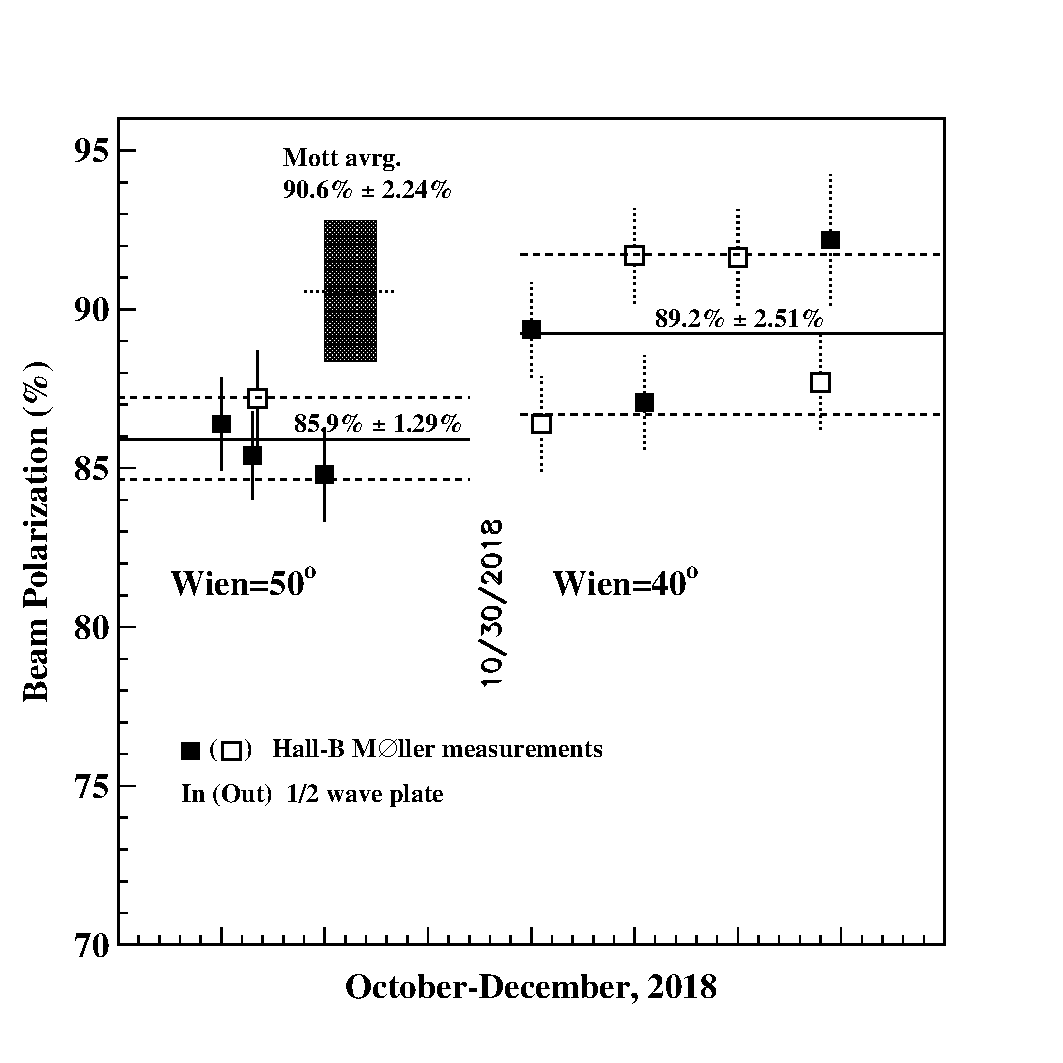
\includegraphics[width=0.5\textwidth]{Moller-RGA-2018.pdf}
\caption{Beam polarization measured in Hall~B during the fall 2018 running period. Prior to October 30 the
  measurements from the Hall~B polarimeter (squares) averaged to $85.9\%\pm1.2\%$ (stat.), which is lower than
  the expected 90\% from the injector Mott measurements (black band). After optimizing the Wien-filter angle the
  average polarization measured in Hall~B was measured to be $89.2\%\pm2.5\%$ (stat.). The filled and open symbols
  correspond to measurements made with and without a half-wave plate, respectively. Error bars are statistical only.}
\label{fig:molrga}
\end{center}
\end{figure}

\begin{figure}[ht]
\begin{center}
\includegraphics[width=0.5\textwidth]{Hall-B_fall_spin_dance.pdf}
\caption{Beam polarization measurements at different Wien angle settings taken during the fall 2018 run period.
  The dashed curve is the cosine-function fit to the data points. The filled point is the average over all measurements
  with the angle set to $50^\circ$ and the open points are from single measurements. Error bars are statistical only. }
\label{fig:sdance}
\end{center}
\end{figure}

Figure~\ref{fig:molrga} has two sets of Hall~B polarimeter measurements done with and without a half-wave plate. The
half-wave plate rotates the electron spin by $180^\circ$. The measurements with and without the the half-wave plate
agree within statistical uncertainties. 


\section{Summary}

The first CLAS12 experiment in 2018 took data successfully at three beam energies; 10.6~GeV, 6.4~GeV, and
2.2~GeV with a liquid-hydrogen target. High quality beam was delivered with a beam size of $< 200$~$\mu$m
and a beam halo as small as 10$^{-4}$ at $5\sigma$ away from the core. The beam position was maintained within
$\sim$200~$\mu$m throughout the run  by the beam feedback system and the fast shutdown system worked in
protecting the CLAS12 detectors from errant beam exposure. With typical M{\o}ller polarimeter runs, the beam
polarization can be measured to an absolute precision of $\sim$2.5\%. 

\section{Acknowledgements}

The authors are grateful for the outstanding efforts by the staff of the Accelerator Division and the Hall~B
Engineering Group at Jefferson Lab during the installation and running of the experiment. We also thank the
CLAS12 Collaboration for manning shifts and taking high quality data. This material is based upon work supported
by the U.S. Department of Energy, Office of Science, Office of Nuclear Physics under contract
DE-AC05-06OR23177 and by the Italian Instituto Nazionale di Fisica Nucleare.

%% The Appendices part is started with the command \appendix;
%% appendix sections are then done as normal sections
%% \appendix

%% \section{}
%% \label{}

%% References
%%
%% Following citation commands can be used in the body text:
%% Usage of \cite is as follows:
%%   \cite{key}          ==>>  [#]
%%   \cite[chap. 2]{key} ==>>  [#, chap. 2]
%%   \citet{key}         ==>>  Author [#]

%% References with bibTeX database:

%\bibliographystyle{model1-num-names}
\bibliographystyle{elsarticle-num}
\bibliography{beamline_nim}
%\bibliography{<your-bib-database>}

%% Authors are advised to submit their bibtex database files. They are
%% requested to list a bibtex style file in the manuscript if they do
%% not want to use model1-num-names.bst.

%% References without bibTeX database:

\end{document}

%%
%% End of file `elsarticle-template-1-num.tex'.
